%%
%% This is file `sample-sigconf-lualatex.tex',
%% generated with the docstrip utility.
%%
%% The original source files were:
%%
%% samples.dtx  (with options: `all,proceedings,bibtex,sigconf')
%% 
%% IMPORTANT NOTICE:
%% 
%% For the copyright see the source file.
%% 
%% Any modified versions of this file must be renamed
%% with new filenames distinct from sample-sigconf-lualatex.tex.
%% 
%% For distribution of the original source see the terms
%% for copying and modification in the file samples.dtx.
%% 
%% This generated file may be distributed as long as the
%% original source files, as listed above, are part of the
%% same distribution. (The sources need not necessarily be
%% in the same archive or directory.)
%%
%%
%% Commands for TeXCount
%TC:macro \cite [option:text,text]
%TC:macro \citep [option:text,text]
%TC:macro \citet [option:text,text]
%TC:envir table 0 1
%TC:envir table* 0 1
%TC:envir tabular [ignore] word
%TC:envir displaymath 0 word
%TC:envir math 0 word
%TC:envir comment 0 0
%%
%% The first command in your LaTeX source must be the \documentclass
%% command.
%%
%% For submission and review of your manuscript please change the
%% command to \documentclass[manuscript, screen, review]{acmart}.
%%
%% When submitting camera ready or to TAPS, please change the command
%% to \documentclass[sigconf]{acmart} or whichever template is required
%% for your publication.
%%
%%
\documentclass[sigconf]{acmart}
%%
%% \BibTeX command to typeset BibTeX logo in the docs
\AtBeginDocument{%
  \providecommand\BibTeX{{%
    Bib\TeX}}}

%% Rights management information.  This information is sent to you
%% when you complete the rights form.  These commands have SAMPLE
%% values in them; it is your responsibility as an author to replace
%% the commands and values with those provided to you when you
%% complete the rights form.
\setcopyright{acmlicensed}
\copyrightyear{2025}
\acmYear{2025}
\acmDOI{XXXXXXX.XXXXXXX}
%% These commands are for a PROCEEDINGS abstract or paper.
\acmConference[]{Schol\'eAI}{ML4ED}{team@schole.ai}
%%
%%  Uncomment \acmBooktitle if the title of the proceedings is different
%%  from ``Proceedings of ...''!
%%
%%\acmBooktitle{Woodstock '18: ACM Symposium on Neural Gaze Detection,
%%  June 03--05, 2018, Woodstock, NY}
\acmISBN{978-1-4503-XXXX-X/2018/06}


%%
%% Submission ID.
%% Use this when submitting an article to a sponsored event. You'll
%% receive a unique submission ID from the organizers
%% of the event, and this ID should be used as the parameter to this command.
%%\acmSubmissionID{123-A56-BU3}

%%
%% For managing citations, it is recommended to use bibliography
%% files in BibTeX format.
%%
%% You can then either use BibTeX with the ACM-Reference-Format style,
%% or BibLaTeX with the acmnumeric or acmauthoryear sytles, that include
%% support for advanced citation of software artefact from the
%% biblatex-software package, also separately available on CTAN.
%%
%% Look at the sample-*-biblatex.tex files for templates showcasing
%% the biblatex styles.
%%

%%
%% The majority of ACM publications use numbered citations and
%% references.  The command \citestyle{authoryear} switches to the
%% "author year" style.
%%
%% If you are preparing content for an event
%% sponsored by ACM SIGGRAPH, you must use the "author year" style of
%% citations and references.
%% Uncommenting
%% the next command will enable that style.
%%\citestyle{acmauthoryear}


%%
%% end of the preamble, start of the body of the document source.
\begin{document}

%%
%% The "title" command has an optional parameter,
%% allowing the author to define a "short title" to be used in page headers.
\title{Federated RLHF Pipeline for Personalized Tutoring}

%%
%% The "author" command and its associated commands are used to define
%% the authors and their affiliations.
%% Of note is the shared affiliation of the first two authors, and the
%% "authornote" and "authornotemark" commands
%% used to denote shared contribution to the research.

\author{J\'er\'emy Chaverot}
\email{jeremy.chaverot@epfl.ch}
\affiliation{%
  {Advised by Vinitra Swamy and Paola Mejia, \\ at the ML4ED lab led by Prof. Tanja K\"aser\\}
  \institution{EPFL, Switzerland}
  \country{}
}

%%
%% The abstract is a short summary of the work to be presented in the
%% article.
\begin{abstract}
  TODO
\end{abstract}


\received{06 June 2025.}
%\received[revised]{12 March 2009}
%\received[accepted]{5 June 2009}

%%
%% This command processes the author and affiliation and title
%% information and builds the first part of the formatted document.
\maketitle

\section{Introduction}

Developped in collaboration with EPFL's ML4ED research lab and recognized by the 2024 Learning Engineering Tools Competition, MIT Solve, and the EPFL Ignition Grant, Schol\'e  AI is a startup committed to transforming the future of online education.

Traditional online platforms like Coursera and edX often suffer from high dropout rates in MOOCs, with figures reaching up to 90\% \cite{warwick65543}. Schol\'e adresses this challenge by offering adult learners personalized, flexible learning experiences. Through multimodal contents, it builds adaptative learning journeys tailored to each individual.

At the core of Schol\'e is Ol\'e, an AI teaching assistant that designs personalized data science learning paths based on your team's specific context. By leveraging cutting-edge research in AI for education, Schol\'e redefines adult upskilling, and ensures learners are equipped for the challenges of tomorrow. However, transforming Ol\'e into an effective AI tutor requires rigorous training and refinement.

 Personalization, scalability, and alignment are critical challenges in educational AI. While large language models have demonstrated strong generative capabilities, aligning their outputs with learner preferences remains a difficult task, particularly when data is distributed and subject to strict privacy constraints.

To address this, we adopt \textsc{FedBiscuit} \cite{wu2025federatedrlhfaggregatedclient}, a recent state-of-the-art framework for federated reinforcement learning with human feedback (RLHF), which we adapt for the context of personalized learning. By leveraging a federated setup, this approach enables preference alignment without centralizing sensitive learner data, ensuring both scalability and privacy.

As Schol\'e is a young startup with limited access to real user interaction data, we rely on large language models to generate high-quality synthetic data representing user preferences. We customize and deploy \textsc{FedBiscuit} on our cluster, applying it to this synthetic data for our personalized learning use case. Our focus is on generating preference pairs and tailored learning curriculums for diverse learner profiles. This work highlights the potential of federated RLHF for scalable, privacy-preserving personalization in low-data settings.

\section{Related Work}

\textbf{LLMs in Education.} The growing accessibility of large language models (LLMs) via platforms such as Hugging Face has opened up new possibilities in education for both learners and instructors \citep{wang2024large}. Students increasingly rely on AI to improve learning efficiency, solve problems, and automate routine tasks, while educators explore ways to enhance teaching strategies and content delivery.

Adaptive learning environments aim to tailor educational content and learning strategies to individual learners' needs, preferences, and performance. To dynamically adjust the learning experience, prior research highlights the importance of user modeling, which means tracking learner behavior, progress, and characteristics. Systems typically adapt content difficulty, feedback, and instructional sequencing to improve engagement and learning outcomes. The integration of intelligent agents has proven effective in managing these personalized adjustments \citep{shih2008adaptive}. This foundational work also supports our project's focus on generating synthetic student profiles and aligning content with diverse learner modalities.

\textbf{Decentralized Training.} Federated learning (FL) \cite{mcmahan2023communicationefficientlearningdeepnetworks} offers a privacy-preserving and communication-efficient solution for training LLMs on decentralized data. Instead of centralizing sensistive datasets, FL enables multiple clients to collaboratively fine-tune a shared model by exchanging only model updates. 

Federated Averaging (FedAvg) \cite{mcmahan2023communicationefficientlearningdeepnetworks}, also refered as Local SGD \cite{stich2019localsgdconvergesfast}, is the standard algorithm in FL. It consists of alternating between a few local
stochastic gradient updates at client nodes, followed by a model averaging update at the server.

Recent frameworks like OpenFedLLM \cite{ye2024openfedllmtraininglargelanguage} have demonstrated the feasability of applying FL to instruction tuning and alignment, two essential components for adapting LLM behavior to user preferences. Using techniques like parameter-efficient fine-tuning (e.g., LoRA \cite{hu2021loralowrankadaptationlarge}), these models can be trained effectively across distributed nodes, and even outperforming centralized baselines in domain-specific tasks. In this project, we adopt this paradigm to align LLMs with learner preferences.

\begin{figure*}
	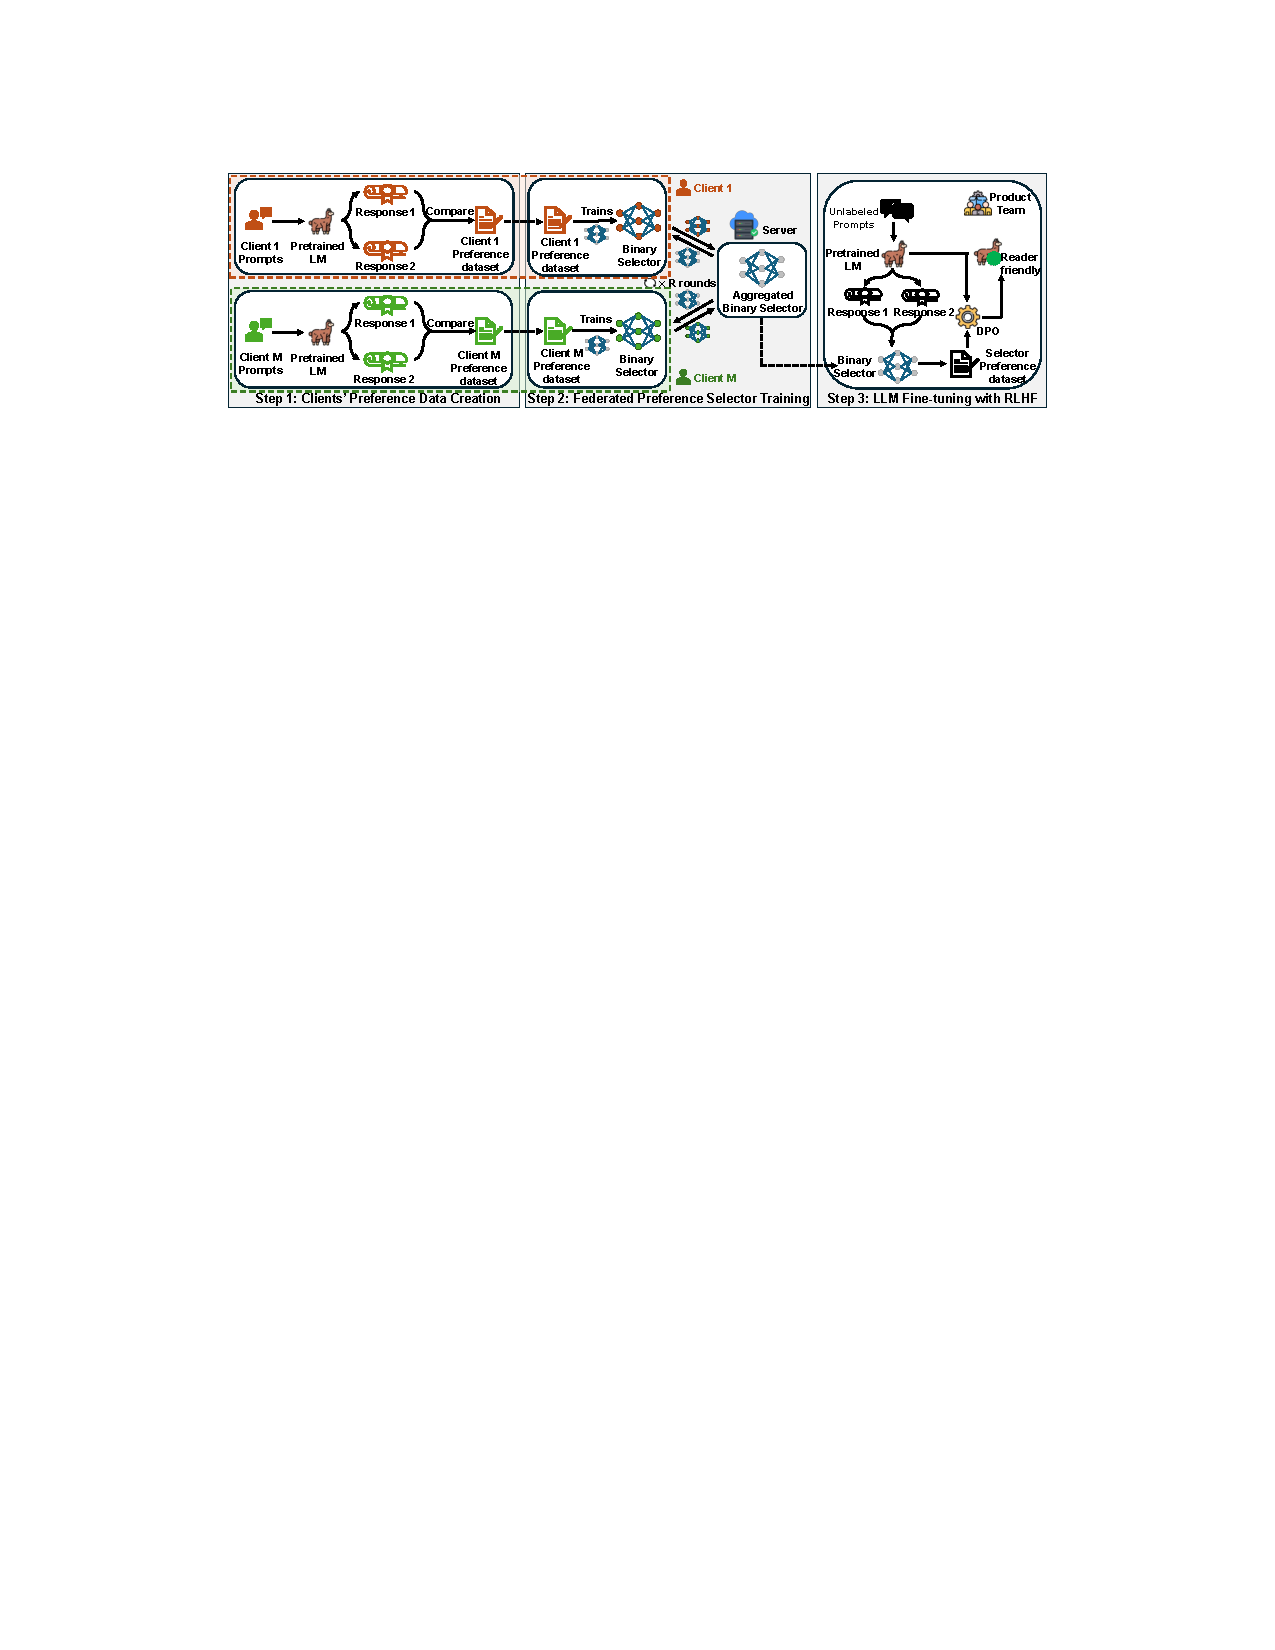
\includegraphics[width=\textwidth]{fedbiscuit-overview}
  \caption{Overview of FedBiscuit.}
  \label{fig:overview}
\end{figure*}

\textbf{Preference Alignment.} Aligning LLMs with human preferences is key to generating pedagogically effective outputs, especially in educational settings where hallucinations or misinterpretations can harm learning \citep{wang2023aligning}. After supervised fine-tuning (SFT), this alignment is typically achieved through RLHF, a family of methods that optimize models based on preference data.

Two main approaches exist within RLHF. The classic RLHF pipeline involves training a reward model to mimic human preferences, followed by reinforcement learning using algorithms like Proximal Policy Optimization (PPO) \citep{schulman2017proximalpolicyoptimizationalgorithms}. While effective, this setup is complex and prone to instability.

In contrast, Direct Preference Optimization (DPO) \citep{Rafailov2023DirectPO} simplifies the process by eliminating the reward model. It directly fine-tunes the base model on preference pairs, optimizing a loss that favors preferred responses. This makes DPO more stable and computationally efficient, while still achieving strong alignment performance \citep{casper2023open}.

For our project, DPO is a better fit: it aligns models directly to learner feedback without requiring a fragile intermediary reward model, and is more suitable for federated training in low-data settings. Moreover, it only requires constructing a dataset of preference pairs (each consisting of a chosen and a rejected learning plan) rather than assigning numerical scores to individual plans, which is more subjective and less straightforward.

\textbf{Synthetic preference and behavioral data} TODO

\section{\textsc{FedBiscuit}}

\textbf{TODO:} Add that FedBiscuit is natively compatible with multi-GPU training and PEFT techniques, great for scalability
\vspace{0.5cm}

\textsc{FedBiscuit} is a state-of-the-art federated reinforcement learning framework designed to align language model behavior with user preferences while preserving user privacy and minimizing communication overhead.

\subsection{Pipeline Overview}
As observed in Figure~\ref{fig:overview}, the pipeline consists of two main training stages. First, clients collaboratively train a binary selector model via federated learning to predict preferences between output pairs (e.g., learning plans). After convergence, the global selector is used to supervise the fine-tuning of the LLM through DPO. For each input, the LLM (e.g., Ol\'e) generates two candidate outputs; the selector picks the preferred one, and DPO updates the LLM accordingly. This avoids the need for a fragile reward model and enables scalable alignment in privacy-sensitive contexts.

\subsubsection{Federated System Design} 
As mentioned earlier, \textsc{FedBiscuit} follows a client-server architecture where, in each communication round, the server distributes the current global model to a subset of selected clients. Each client then fine-tunes the model locally using its own preference data. Once local training is complete, the clients send back their model updates, which the server aggregates to form an updated global model. This iterative process continues until convergence or until a predefined number of rounds has been reached.

\subsubsection{Client-Side Operations} 
On the client side, each participant preprocesses their data to construct training samples in the form of preference pairs (i.e., chosen vs. rejected responses to a given prompt). In our adaptation for educational personalization, these preference pairs correspond to selected and discarded learning plans given the student behavioral data and preferences. Local models are trained as a classification task using the cross-entropy (CE) loss $l_{CE}$.
\begin{equation}
	l_{CE}= ...
\end{equation}

\subsubsection{Server-Side Aggregation} 
The central server aggregates model updates without ever accessing raw client data, only model weights or gradients are exchanged. This is enabled by a secure aggregation mechanism, which guarantees that the server can only see the final aggregated result \cite{bonawitz2016practicalsecureaggregationfederated}. The server also handles client sampling and adapts dynamically to slower or disconnected clients during training.

\begin{equation}
	aggregation \;\; formula
\end{equation}

\subsubsection{LLM-as-a-Judge Evaluation} 
To evaluate alignment, \textsc{FedBiscuit} leverages Auto-J, a 13B-parameter generative language model specifically trained to assess other models through natural language critiques. Developed using large-scale user queries and LLM responses, Auto-J achieves competitive performance across 58 real-world evaluation scenarios. In the context of Schol\'e, Auto-J is particularly valuable: it provides an automated, scalable, and interpretable means of assessing how well Ol\'e aligns with learner preferences, without relying on expensive human annotations or black-box evaluators.

\subsection{Use Case and Limitations} 
\subsubsection{TL;DR Summarization Task} To benchmark alignment performance, \textsc{FedBiscuit} uses the TL;DR summarization task, which consists in generating concise summaries of Reddit posts. This controlled setup helps evaluate preference learning and is later used to estimate the amount of data each client needs in educational settings like for Schol\'e.

\subsubsection{Limitations} 
Despite its strengths, \textsc{FedBiscuit} happens to face some limitations. First, communication overhead remains a bottleneck, especially as the number of clients increases. Second, the system's effectiveness can degrade in the presence of extreme client heterogeneity, both in data quality and hardware capabilities. Finally, the current framework assumes clients have enough data to perform meaningful updates, which may not hold in sparse real-world scenarios. 

In our specific setup, some of these challenges are mitigated. We assume client training occurs on the same server-side machine, removing issues related to hardware variation and network latency. While this setup compromises some of the privacy advantages offered by \textsc{FedBiscuit}, it enables us to establish a strong baseline with full control over the hardware environment. As for data sparsity, this work also introduces methods to generate synthetic data and augment existing datasets, providing a practical solution for low-data scenarios like those found for Schol\'e use case.


\section{Synthetic Data Generation and Evaluation}

As Schol\'e AI is still in its early development phase, we currently do not have access to real-world user data. To lay the foundation for experimentation and model training, we first established a formal typology of the types of data that will characterize student profiles. We categorized the data into two primary types: explicit data and implicit data.

\paragraph{Explicit Data.}  
This category encompasses all directly stated learner preferences and declared learning goals. It includes information such as preferred learning modalities, self-reported motivation, goal orientation, or feedback explicitly given by the learner regarding content relevance or difficulty. These data points are directly interpretable. The detailed categories can be found in Appendix~\ref{appendix:explicit_data}.

\paragraph{Implicit Data.}  
Also referred to as \textit{behavioral data}, this category includes information derived from the learner's interaction patterns with the learning system. Behavioral data captures observable signals such as time spent on tasks, content navigation paths, click-through rates, quiz completion rates, and error frequencies. The detailed categories can be found in Appendix~\ref{appendix:implicit_data}.

\subsection{Prompt Engineering}

\subsubsection{System prompt} The system prompt is responsible for guiding the model by specifying the overall structure, formatting, and style of the generated output. Unlike the user prompt, it remains constant across generations.

We implemented a synthetic data generation pipeline built upon prompt engineering techniques, following the methodology presented in \cite{sahoo2025systematicsurveypromptengineering}. We adopted the   \textbf{in-context learning} (ICL) \cite{dong2024surveyincontextlearning} with \textbf{one-shot prompting}, enabling the model to produce with simplicity structured and context-aware outputs. 

\textit{In-context learning} is a paradigm that allows language models to learn tasks given only a few examples in the form of demonstration. This allows the model to adapt its behavior based on the structure and semantics of the provided context. In \textit{One-shot prompting}, the model is given a single example before generating a new output.

Each system prompt is structured as follows:
\begin{itemize}
    \item A subgraph extracted from Schol\'e AI's main \textit{knowledge graph} (KG) \textbf{TODO: add how it was extracted}, describing learning modules. This ensures that the model grounds its generation in the actual curriculum.
    \item A strict requirement to output data in a structured \texttt{JSON} format, which enables automatic validation and downstream processing.
    \item A combination of learning modality and student profile to guide personalization and diversity in the synthetic data.
\end{itemize}

\subsubsection{User prompt} To introduce diversity in the generated data, we incorporate personalization into the user prompt with the learning modality and student profile. This prompt also specifies the number of generations to produce.

\paragraph{Learning Modalities.}  
We defined the following learning modalities to reflect common cognitive styles according to the VARK model:

{\small
\begin{itemize}
    \item \textit{Visual}: prefers diagrams, illustrations, and video content.
    \item \textit{Auditory}: favors spoken explanations, podcasts, and discussions.
    \item \textit{Reading/Writing}: learns through text-based material such as articles and notes.
    \item \textit{Kinesthetic}: benefits from interactive, hands-on experiences.
\end{itemize}
}

It's worth noting that these modalities can be somewhat controversial, which is why they should be used with caution \cite{vark-casestudy}. Nonetheless, we adopt them in the early stages due to their simplicity.

\paragraph{Student Profiles.}  
We define several learner types to reflect diverse engagement styles:

{\small
\begin{itemize}
\item \textit{Goal-Oriented}: driven by milestones and performance tracking.
\item \textit{Curious}: explores optional content and asks open-ended questions.
\item \textit{Passive}: minimal engagement, avoids extra effort.
\item \textit{Fast-Paced}: skims content, prioritizes speed over depth.
\item \textit{Confused}: struggles with core concepts, needs clear guidance.
\item \textit{Struggling}: performs poorly, benefits from scaffolding and feedback.
\item \textit{Social}: learns through discussion and peer interaction.
\end{itemize}
}

In particular, for tasks such as data augmentation and generation of learning curriculum preferences, the model is explicitly instructed to interpret the given learner context and adjust its outputs accordingly. For example, a kinesthetic-exploratory learner may be recommended simulations and interactive labs, while a visual goal-oriented learner may receive structured video tutorials and milestone-based feedback.


\textbf{TODO:} Add diagram to summarize prompt structure

The latest versions of the prompts are available at \href{https://github.com/JCHAVEROT/semester-project/tree/main/experiments/SyntheticData/prompts}{this link}.

\subsection{Streamlit Interface for Prompt Interaction}

To support fast iterations on prompt design and inference control, we developed an interactive interface using \textbf{Streamlit}.

\textit{Streamlit} is an open-source Python framework that enables rapid development of web applications for data science and machine learning tasks. It allows users to manipulate model inputs and visualize outputs without requiring front-end development.

Our Streamlit interface provides the following features:
\begin{itemize}
	\item Choosing the task type.
	\item Editing prompt content in real time.
	\item Selecting learning modalities and student profiles.
	\item Evaluating the generated synthetic data.
% \item Adjusting generation parameters such as temperature, top-$p$, and model choice.
\end{itemize}

The website can be accessed at this link: \href{https://scholeai-data-generation.streamlit.app/}{https://scholeai-data-generation.streamlit.app/}

\vspace{0.5cm}
\textbf{TODO:} Add screenshots

\subsection{Evaluation Pipeline: Automated and Human-in-the-Loop}

Once the synthetic data pipeline was functional, the next challenge was to assess the quality of the generated outputs. We implemented a two-tiered evaluation process combining automated validation and human annotation.

\subsubsection{Automated Evaluation}  
Given the structured nature of the outputs, we first applied a series of automated validation tests to each generated \texttt{JSON} sample. These included the following checks, among others:
\begin{itemize}
    \item All required fields were present and of the correct type.
    \item Categorical values (e.g., learning modality) belonged to the expected set.
    \item Text fields were non-empty where applicable.
    \item Timestamps respected ISO 8601 formatting and logical sequencing.
    \item Numeric ratings fell within predefined bounds (e.g., 1--5).
\end{itemize}

These tests served as an efficient first-pass filter, rejecting malformed samples before any human review.

\subsubsection{Human Evaluation via Yes-No Questions}  
For semantic and pedagogical validity, we developed a human annotation interface embedded on the Streamlit web app. Annotators assessed each sample using a series of \textit{yes-no questions}, such as:
\begin{itemize}
    \item Is the proposed curriculum realistic for the given student profile?
    \item Does the plan match the specified learning modality?
    \item Is the behavioral data coherent and believable?
\end{itemize}

This human-in-the-loop component allowed for rapid, structured assessment without requiring full expert review. The feedback was used to iteratively improve prompt design and increase generation quality. The full list of questions is provided in Appendix~\ref{appendix:questions}.

\subsubsection{Visualization of Evaluation Results}  
To monitor performance and guide refinements, we used librairy Plotly to produce interactive dashboards summarizing evaluation statistics for automated checks and human questions.
These summaries help understand what is working or not in the prompts and make it easier to track changes over time.

\textbf{TODO:} Add screenshot and some stats

\subsection{Challenges in Synthetic Data Generation}

The combined evaluation process surfaced several key insights. Using GPT-4o-mini as the generating model, automated validation revealed high structural correctness in most cases. However, as the number of generated samples increases, structural errors (such as malformed \texttt{JSON}) become more frequent. This is likely due to the verbosity of the syntax, where even a small mistake (e.g., a missing comma) can break the entire structure. Switching to a more lightweight format like \texttt{YAML} could help mitigate this. Alternatively, using a framework like LMQL \cite{Beurer_Kellner_2023}, which enables constrained generation through embedded code logic, could enforce correct output structure regardless of sample count.

Beyond structural issues, semantic inconsistencies were more prevalent. These included unrealistic behavioral traces, such as improbable activity sequences or timestamp patterns that did not reflect plausible learner behavior.

These challenges highlight the limitations of LLM-based generation, particularly when prompt conditioning is weak or underspecified. They underscore the need for clear in-context examples for format control, and a multi-layer evaluation process to ensure data quality. Notably, LMQL could be a promising solution for addressing both structural and semantic reliability during generation.

\textbf{TODO:} Add examples of malformed samples

\section{Experiment}
\begin{itemize}
    \item TL;DR summarization task as baseline for system validation.
    \item Objective: Identify optimal training dataset size and configuration.
    \item Simulation setup: client number, synthetic dataset distribution.
    \item Tested model architectures and size variations.
    \item Explored hyperparameters: federated rounds, learning rates, batch sizes.
    \item Hardware specifications
    \item Use of Weight\&Biases to monitor trainings.
 	\item Challenges
\end{itemize}


\section{Results}
\begin{itemize}
    \item Quantitative metrics
    \item Comparative analysis of simulation configurations and dataset sizes
    \item Visualizations: graphs or barplots
    \item In-depth analysis: student preference alignment, edge cases, anomalies
    \item Interpretation of results in federated learning context and practical implications.
\end{itemize}

\section{Conclusion and Future Work}
\begin{itemize}
    \item Summary of achieved goals and core contributions in federated RLHF for education
    \item What can be improved
    \item Potential next steps: deployment with real student data, model scalability improvements
    \item Directions for future research: (ideas: real-time feedback integration, adaptive learning paths, constrained inference for synthetic data)
\end{itemize}

%%
%% The acknowledgments section is defined using the "acks" environment
%% (and NOT an unnumbered section). This ensures the proper
%% identification of the section in the article metadata, and the
%% consistent spelling of the heading.
%\begin{acks}
%TBD
%\end{acks}

%%
%% The next two lines define the bibliography style to be used, and
%% the bibliography file.
\bibliographystyle{ACM-Reference-Format}
\bibliography{sample-base}


%%
%% If your work has an appendix, this is the place to put it.
\appendix


\section{Explicit Data Categories}
\label{appendix:explicit_data}

The following list describes the categories of explicit data used to characterize Schol\'e AI learners. These data points are directly provided by the user or derived from user feedback and preferences.
{\footnotesize
\begin{itemize}
    \item \textbf{ratings\_on\_modules}: User ratings on the effectiveness and quality of learning modules.
    \item \textbf{approval\_of\_content\_modifications}: Whether the user accepted or rejected system-suggested changes.
    \item \textbf{explicit\_learning\_goals}: Stated learning goals or objectives provided by the user.
    \item \textbf{initial\_curriculum\_state}: Ordered list of module names representing the system-suggested curriculum before any user modifications.
    \item \textbf{drag\_and\_drop\_curriculum\_edits}: Reordering of the learning path via drag-and-drop (track index changes).
    \item \textbf{curriculum\_editing\_feedback}: Feedback provided after modifying the suggested curriculum.
    \item \textbf{preferred\_content\_format}: User preference among text, video, or audio content.
    \item \textbf{reflection\_inputs}: Written explanations for curriculum modifications or preferences.
    \item \textbf{satisfaction\_surveys}: Survey responses about overall platform satisfaction.
    \item \textbf{skill\_self\_assessments}: Self-evaluated skill level before and after learning sessions.
    \item \textbf{relevance\_feedback}: Feedback about whether the content matched the user's real-world needs (Likert scale 1-5).
    \item \textbf{difficulty\_feedback}: Perceived difficulty level of content (Likert scale 1-5).
    \item \textbf{trust\_feedback}: Degree of trust in the platform's tutoring and recommendations (Likert scale 1-5).
\end{itemize}
}

\section{Implicit Data Categories}
\label{appendix:implicit_data}

The following list describes the categories of implicit data collected from user interactions on Schol\'e AI. These signals are inferred from behavior and engagement patterns.

{\footnotesize
\begin{itemize}
    \item \textbf{timestamped\_clicks}: List of all clicks with timestamps (e.g., button presses, navigation).
    \item \textbf{scrolling\_behavior}: Scrolling depth, speed, and frequency during content consumption.
    \item \textbf{time\_on\_task\_per\_module}: Duration a user spends on each learning module or page.
    \item \textbf{skipped\_modules}: List of modules that were skipped by the user.
    \item \textbf{engagement\_metrics}: Completion rates, frequency of activity, interaction levels.
    \item \textbf{pace\_tracking\_signals}: Estimated learning speed from knowledge tracing (e.g., fast vs slow pace).
    \item \textbf{drop\_off\_events}: Points where users abandon a module or quit mid-session.
    \item \textbf{content\_adaptation\_requests}: Requests made by users to adjust difficulty or format.
    \item \textbf{memory\_usage\_patterns}: Tracking usage of personalized memory features (e.g., saved preferences).
    \item \textbf{interactions\_with\_tutor}: Timestamps, questions, and responses during tutor interactions.
    \item \textbf{number\_of\_retries\_on\_quizzes}: Number of attempts needed to successfully complete quizzes.
    \item \textbf{response\_times}: Time taken to answer questions or to interact after prompts.
\end{itemize}
}

\section{Human Evaluation Questions}
\label{appendix:questions}

The following yes/no questions were used by human evaluators to assess the quality and realism of the synthetic student data:

{\footnotesize
\begin{itemize}
    \item \textbf{QH1.} Do the user behaviors feel realistic and consistent with the assigned student profile?
    \item \textbf{QH2.} Does the sequence of actions and timestamps reflect plausible learning behavior over time?
    \item \textbf{QH3.} Is the generated content (e.g., goals, reflections, preferences) coherent and appropriate given the context?
    \item \textbf{QH4.} Do the interactions with the AI tutor sound natural and relevant to the user's learning progress?
    \item \textbf{QH5.} Does the data reflect meaningful variation across different users or profiles?
    \item \textbf{QH6.} Is there any repetition or redundancy that feels unnatural or overly templated?
    \item \textbf{QH7.} Do the initial curriculum and the user's edits (e.g., module reordering or removals) make sense and align with the learner's profile?
    \item \textbf{QH8.} Would this data be convincing if presented as part of a real learner's interaction log?
\end{itemize}
}

\end{document}
\endinput
%%
%% End of file `sample-sigconf-lualatex.tex'.
